\section{Generalization \& Sequential Exchangeability}
\label{sec: seq_exchangeability_alt_design}

In this section, we develop the concept of \emph{sequential exchangeability}, extending the original assumptions stated in Theorem \ref{theorem: identify_cwsd}. This extension is motivated by the observation that carryover effects are not unique to \cwsd{} but can also influence inference in other sequential experimental designs.

For instance, in \cite{09_Clifford}, the authors advocated for the adoption of pre-post designs, wherein participants are initially exposed to a control condition before transitioning to a between-subjects design. They posited that this approach enhances precision. However, in one of the experiments they replicated, carryover effects appeared to influence inference—not necessarily in the direction of the effect, but rather in its magnitude.

Experiment 2 in \cite{09_Clifford} replicated a landmark study on foreign aid by \citep{GilensMartin2001PIaC}, investigating the influence of factual information regarding federal budget allocation for foreign aid on public opinion. In that study, respondents were informed that spending on foreign aid constituted less than 1\% of the federal budget, after which they were asked whether foreign aid spending should be increased or decreased, with responses recorded on a five-point scale.

To compare different experimental designs, participants were randomly assigned to one of two conditions: the \textit{post-only} design or the \textit{pre-post} design. In the \textit{post-only} design, participants were randomized to receive the budgetary information, consistent with a between-subjects approach. Conversely, in the \textit{pre-post} design, participants first provided their opinion on foreign aid without the budgetary information, were subsequently exposed to the budgetary information, and finally responded to the same question again. The results of this replication indicate substantial differences in the estimated effects, as depicted in Figure \ref{fig:difference-in-estimates_clifford}.

\begin{figure}[h]
    \centering
    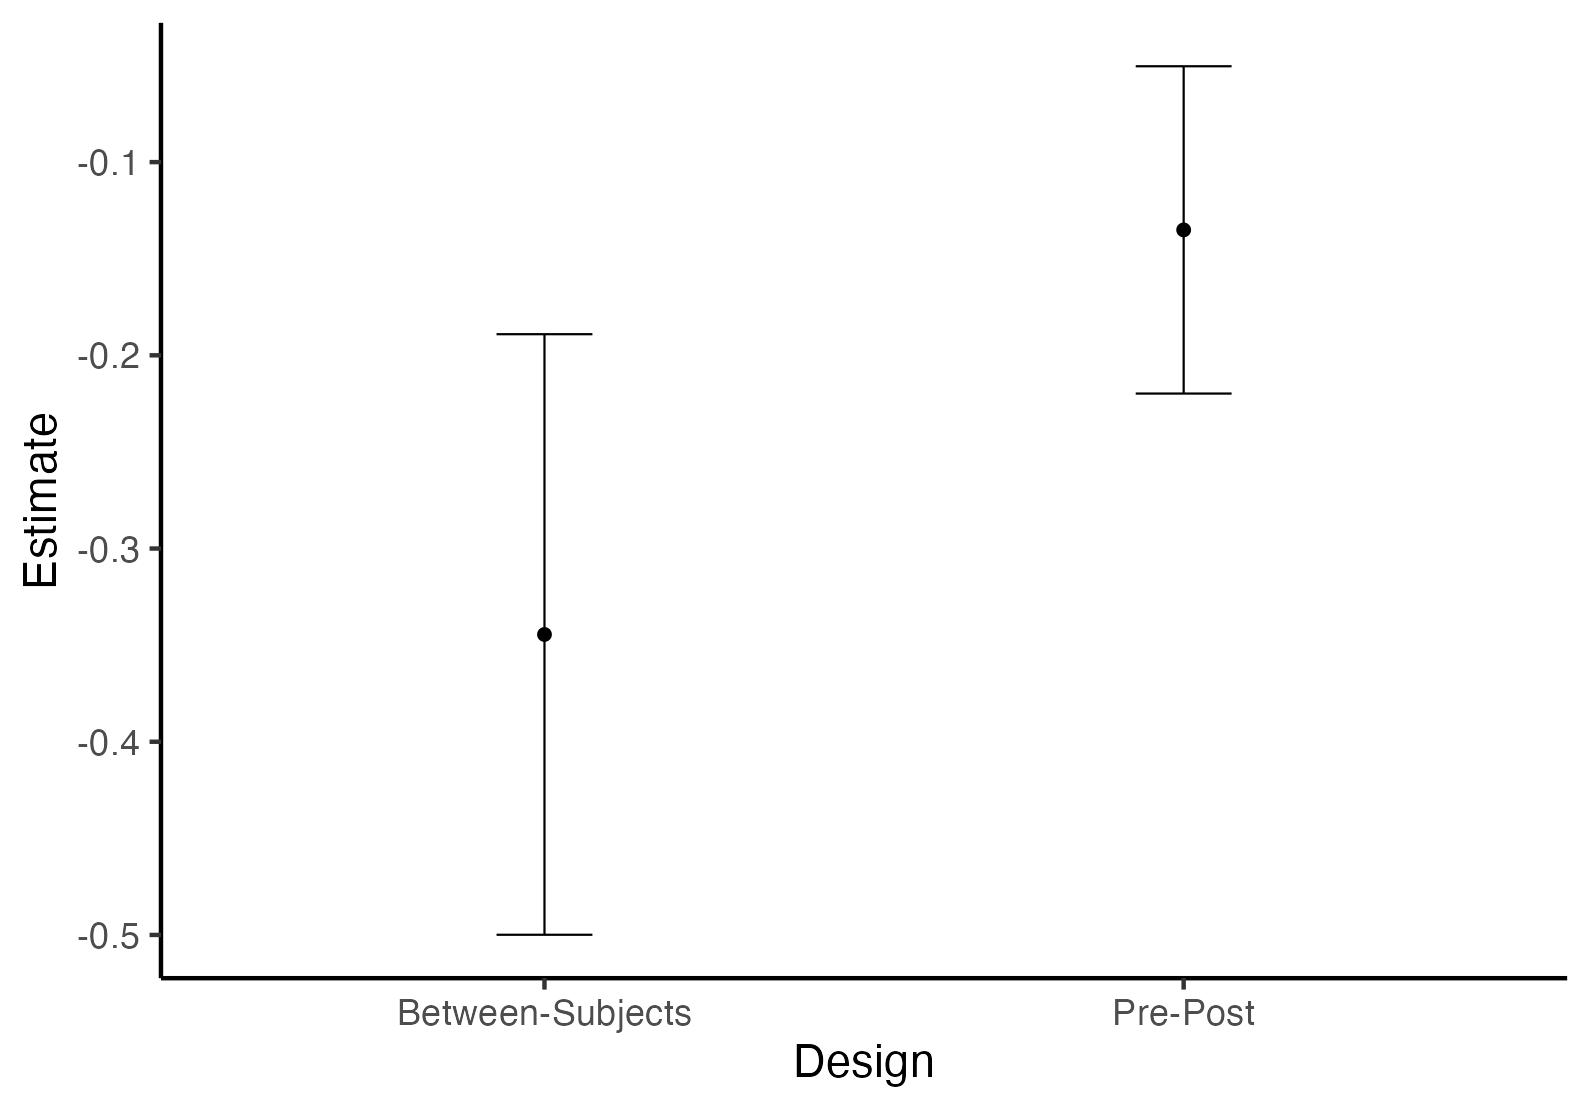
\includegraphics[width=0.75\linewidth]{Figures/estimates.jpg}
    \caption{Experiment 2 in \cite{09_Clifford}}
    \label{fig:difference-in-estimates_clifford}
\end{figure}

This example demonstrates how experimental design choices can markedly affect inference. Specifically, it suggests that the estimated treatment effect varies with the design, potentially due to carryover effects. Formally, we observe that:
\[
 \tau^{\text{between-subjects}} = \mathbb{E}[Y_i(1) - Y_i(0)] \neq \tau^{\text{pre-post}} = \mathbb{E}[Y_i(0,1) - Y_i(0,0)]
\]
Thus, the notion of \emph{sequential exchangeability} provides a framework to examine the conditions under which these two estimands may be equivalent.

\subsection{Sequential Exchangeability}

In the \cwsd{} design, the sequence in which participants receive the treatment or control is randomized such that $Z_{i,t_1}$ determines $Z_{i,t_2}$; specifically, $Z_{i,t_1} = 1 - Z_{i,t_2}$. In contrast, the pre-post design employed in Experiment 2 in \cite{09_Clifford} randomizes participants' treatment status at time $t_2$, with all participants receiving the control in time $t_1$.

Moreover, other sequential experimental designs randomize treatment assignment in both time periods, as will be discussed further in Section \ref{section: alternative_designs}. In order to generalize, we can redefine Equation \ref{equation: t2_identity_cwsd} as follows:
\begin{equation}
\label{equation: t2_identity} 
    Y_{i,t_2}^{\text{obs}} = \sum_{z_{i,t_1} \in \{0,1\}} \sum_{z_{i,t_2} \in \{0,1\}} Y_{i,t_2}(z_{i,t_1}, z_{i,t_2})\,\mathbbm{1}\{Z_{i,t_1} = z_{i,t_1}\}\,\mathbbm{1}\{Z_{i,t_2} = z_{i,t_2}\}.
\end{equation}

\noindent
We now formally define \emph{sequential exchangeability} as follows:

\begin{assumption}(Sequential Exchangeability)
\label{assumption: sequential_exchangeability}
 A sequential experimental design with two time periods and two treatment conditions satisfies \emph{sequential exchangeability} if the following conditions are met:
    \begin{assumptionnum}
        \item \label{assumption: sequential_exchangeability: controlled_carryover} 
        \textbf{Controlled carryover effects: } 
        \[
        Y_{i,t_2}(z_{i,t_1}, z_{i,t_2}) = Y_{i,t_2}(z_{i,t_2}) \mid Z_{i,t_1} = z_{i,t_1}, Z_{i,t_2} = z_{i,t_2}, X_{i,t_2}, \quad \forall z_{i,t_1}, z_{i,t_2} \in \{0,1\}
        \] 

        \item \label{assumption: sequential_exchangeability: ignorability_t2} 
        \textbf{Ignorability at time $t_2$:} 
        \[
        Y_{i,t_2}(z_{i,t_2}) \indep  Z_{i,t_2} \mid X_{i,t_2}, \quad  \forall z_{i,t_2} \in \{0,1\}.
        \]
        \item \label{assumption: sequential_exchangeability: parallel_trend} 
        \textbf{Parallel trend assumption:} 
        \[
        Y_{i,t_2}(z_{i,t_2}) = Y_{i,t_1}(z_{i,t_2}) + c, \quad \forall z_{i,t_2} \in \{0,1\},\ c \in \mathbb{R}.
        \]
    \end{assumptionnum}
    These conditions are considered in addition to SUTVA and the overlap assumptions stipulated by the Rubin Causal Model.
\end{assumption}

\noindent 
The generalization to $n$ time periods and $n$ conditions can be found in the Appendix.

The primary distinction between \emph{sequential exchangeability} and the assumptions required to identify the average treatment effect (ATE) in \cwsd{} lies in Assumption \ref{assumption: sequential_exchangeability: controlled_carryover}. Intuitively, if carryover effects can be appropriately controlled—such that the potential outcome at $t_2$ corresponds to that which would be observed if the participant were recruited at $t_2$ without any prior intervention. We want to note however that this is a \emph{strong} assumption that can be easily violated. We explore some of the practical challenges in controlling for the direct carryover effects in Section \ref{sec: control_carryover_eff_challenges}.

Evaluating Experiment 2 in \cite{09_Clifford} with respect to Assumption \ref{assumption: sequential_exchangeability}, it is plausible that Assumptions \ref{assumption: sequential_exchangeability: ignorability_t2} and \ref{assumption: sequential_exchangeability: parallel_trend} hold, given that participants were randomized at $t_2$ and the parallel trend assumption seem plausible. However, due to the nature of the experiment, administering the question at $t_1$ may introduce carryover effects that are challenging to control for. The mechanism by which treatment at $t_1$ influences the outcome at $t_2$ is ambiguous, thereby potentially violating Assumption \ref{assumption: sequential_exchangeability: controlled_carryover}.

\subsection{Alternative Sequential Experimental Designs}
\label{section: alternative_designs}

Based on the sequential exchangeability assumptions, we propose several alternative experimental designs to \cwsd{} that may be more appropriate in contexts where the underlying assumptions are more plausible. Although these designs have been previously employed for diverse purposes as noted in the introduction, our focus here is on their utility for estimating the average treatment effect (ATE).

\begin{figure}[h]
    \centering
    \begin{subfigure}[b]{0.45\textwidth}
    \resizebox{\textwidth}{!}{%
    \fbox{
    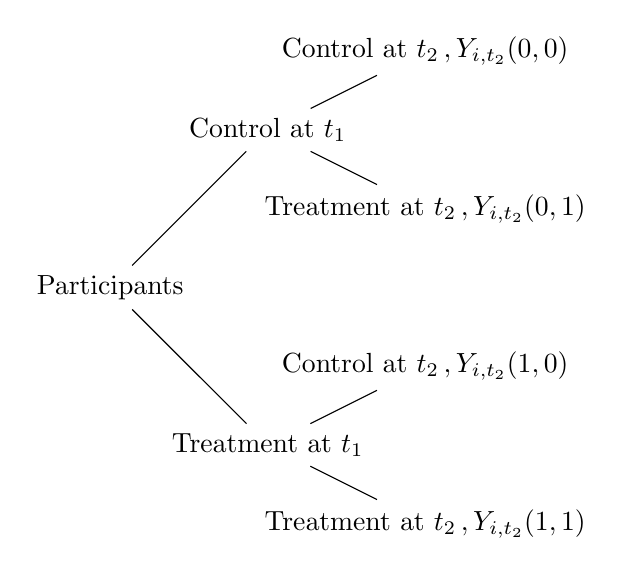
\begin{tikzpicture}[
  grow=right,
  level 1/.style={sibling distance=4cm, level distance=2cm},
  level 2/.style={sibling distance=2cm, level distance=2cm}]
    % Root node representing the experiment
    \node {Participants}
     % First randomization at t1 (first time period)
    child { node {Treatment at \(t_1\)}
    % Second randomization at t2 for first branch
    child { node {Treatment at \(t_2 \,, Y_{i,t_2}(1,1)\)} }
    child { node {Control at \(t_2 \,, Y_{i,t_2}(1,0)\)} }
    }
    % Second branch from the first randomization at t1
    child { node {Control at \(t_1\)}
    % Second randomization at t2 for second branch
    child { node {Treatment at \(t_2 \,, Y_{i,t_2}(0,1)\)} }
    child { node {Control at \(t_2 \,, Y_{i,t_2}(0,0)\)} }
  };
\end{tikzpicture}}
}
\subcaption{Sequential Randomization}
\label{fig:alt_designs_both}
\end{subfigure}
\hspace{10mm}
\begin{subfigure}[b]{0.45\textwidth}
\resizebox{\textwidth}{!}{%
\fbox{
    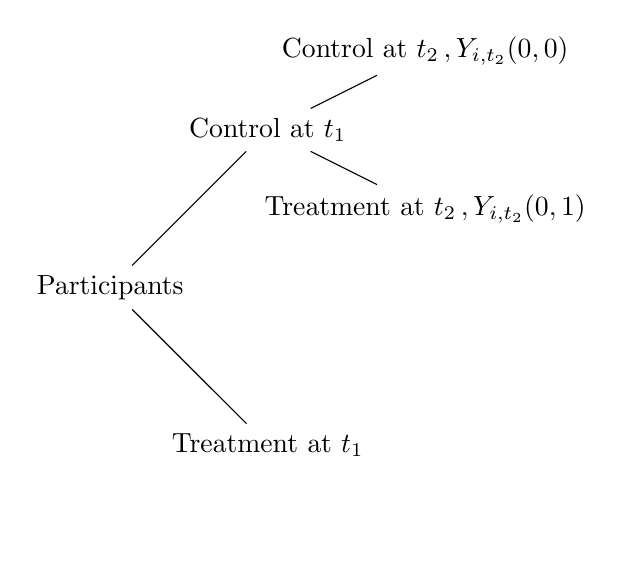
\begin{tikzpicture}[
  grow=right,
  level 1/.style={sibling distance=4cm, level distance=2cm},
  level 2/.style={sibling distance=2cm, level distance=2cm}],
    % Root node representing the experiment
    \node {Participants}
    child { node {Treatment at \(t_1\)}
    % Second randomization at t2 for first branch
    child { node {} edge from parent[draw=none] }
    child { node {} edge from parent[draw=none] }
    }
    % Second branch from the first randomization at t1
    child { node {Control at \(t_1\)}
    % Second randomization at t2 for second branch
    child { node {Treatment at \(t_2 \,, Y_{i,t_2}(0,1)\)} }
    child { node {Control at \(t_2 \,, Y_{i,t_2}(0,0)\)} }
  };
\end{tikzpicture}}
}
\subcaption{Selective Sequential Randomization}
\label{fig:alt_designs_selective}
\end{subfigure}
    \caption{Alternative Experimental Designs to \Cwsd{}}
    \label{fig:alt_designs}
\end{figure}

A notable advantage of the sequential randomization design depicted in Figure \ref{fig:alt_designs_both} is its ability to incorporate \(Z_{i,t_1}\) as a control variable without introducing perfect collinearity. In traditional \cwsd{} settings, the deterministic relationship \(Z_{i,t_1} = 1 - Z_{i,t_2}\) renders it infeasible to include both treatment indicators in an OLS regression model. By contrast, the sequential randomization design circumvents this issue, thereby allowing more robust estimation strategies. Nonetheless, a key challenge remains in accurately characterizing the nature of carryover effects; the risk of misspecification looms large if these effects are not thoroughly understood.

The most significant benefit of the proposed experimental designs is the credibility of the ignorability assumption at time \(t_2\) (Assumption \ref{assumption: sequential_exchangeability: ignorability_t2}). When randomization is implemented independently in the second stage, the potential for unobserved confounding—particularly through indirect carryover effects—is substantially reduced. This is especially valuable since  experimental designs are often applied to estimate the average treatment effect, without assuming how potential covariates might confound the estimate. 

Sequential experimental designs can and should be carefully tailored to the specific context of an experiment. For instance, consider the selective sequential randomization design illustrated in Figure \ref{fig:alt_designs_selective}. If carryover effects are negligible in one of the conditions—such as when the control involves a placebo (e.g., a sugar pill assumed to have no effects of the outcome of interest)—then it may be reasonable to relax Assumption \ref{assumption: sequential_exchangeability: controlled_carryover}, where the assumption is true for \(z_{i,t_1} = 0\) but not \(z_{i,t_1} = 1\). In this scenario, the selective design could yield reliable ATE estimates. However, if the control represents a current standard treatment and the experimental arm involves a novel intervention, where both conditions may have significant carryover effects, relaxing the assumption would be inappropriate, as the differential impact of prior exposure could bias the estimation of ATE. This emphasis on accounting for the nature of the experiment and treatment, and on adapting the randomization of treatment assignment for causal identification, echoes the rationale behind dynamic treatment regimes and Sequential Multiple Assignment Randomized Trial (SMART) designs, which similarly account for sequential assignments to estimate causal effects under minimal modeling assumptions \citep{25_SMARTDesign}.

For completeness, we state the following corollary linking sequential exchangeability to the validity of the proposed experimental designs.

\begin{cor}
\label{cor: two-period-two-arm}
  In \emph{any} two‐period, two‐arm sequential experimental design, if \emph{sequential exchangeability}
  holds, then
  \[
    \tau_{t_2}^{\mathrm{seq}} \;=\; \tau.
  \]
\end{cor} 

The proof proceeds analogously to that of Theorem \ref{theorem: identify_cwsd}.

\begin{remark}
  Equation \ref{equation: t2_identity} in fact provides the most general two‐period, two‐arm sequential‐outcome set‐up that includes counterbalanced within‐subjects designa, the pre–post designs, sequential randomization designs,  selective sequential randomization designs, if \emph{sequential exchangeability}
  holds, then
  \[
    \tau_{t_2}^{\mathrm{seq}} \;=\; \tau.
  \] Hence whenever the observed second‐period outcome in your design can be written in this form, the proof of Corollary \ref{cor: two-period-two-arm} goes through verbatim under the sequential exchangeability assumption. 
\end{remark}

\subsection{Controlling for Carryover Effects in Practice}
\label{sec: control_carryover_eff_challenges}

Carryover effects from the treatment at time $t_1$ can be viewed as a form of omitted variable bias—essentially, a `covariate' that needs to be properly accounted for. As with any covariate, misspecifying its functional form can lead to biased estimates. If carryover effects are linearly separable, then a fixed-effects model that includes treatment status at $t_1$ as a control is typically sufficient. However, when carryover effects interact with the subsequent treatment at $t_2$, estimation becomes more complex.

Consider two illustrative models where carryover effects cannot be fully addressed by simple fixed-effects approaches. If the carryover effects from $t_1$ interacts outcomes at $t_2$ in an additive way, we can model the outcome as:

\begin{equation}
\label{eq: interaction_carryover}
Y_{i,t_2} 
= \beta_0 + \beta_1 Z_{i,t_2} 
+ \gamma (Z_{i,t_1} \cdot Z_{i,t_2}) 
+ \beta_2 X_{i, t_2} 
+ \epsilon_{i, t_2}, 
\quad \epsilon_{i, t_2} \sim N(0,\sigma^2).
\end{equation}

Here, the effect of the second treatment $Z_{i,t_2}$ depends additively on whether the first treatment $Z_{i,t_1}$ was received, through the interaction term $\gamma (Z_{i,t_1} \cdot Z_{i,t_2})$.

If, instead, the prior treatment amplifies or dampens the effect of the later treatment in a nonlinear way—as in the following model:
\begin{equation}
\label{eq: compounding_carryover}
Y_{i,t_2} 
= \beta_0 
+ \beta_1^{1 + \gamma Z_{i,t_1}} Z_{i,t_2} 
+ \beta_2 X_{i,t_2} 
+ \epsilon_{i, t_2}, 
\quad \epsilon_{i, t_2} \sim N(0,\sigma^2).
\end{equation}
In this formulation, the strength of the effect of \( Z_{i,t_2} \) is modulated by prior exposure \( Z_{i,t_1} \) through an exponentiated function. When \( \gamma > 0 \), prior treatment increases the effective coefficient on \( Z_{i,t_2} \), amplifying its influence on the outcome. Conversely, when \( \gamma < 0 \), the coefficient is dampened. 


\begin{figure}[h]
    \centering
    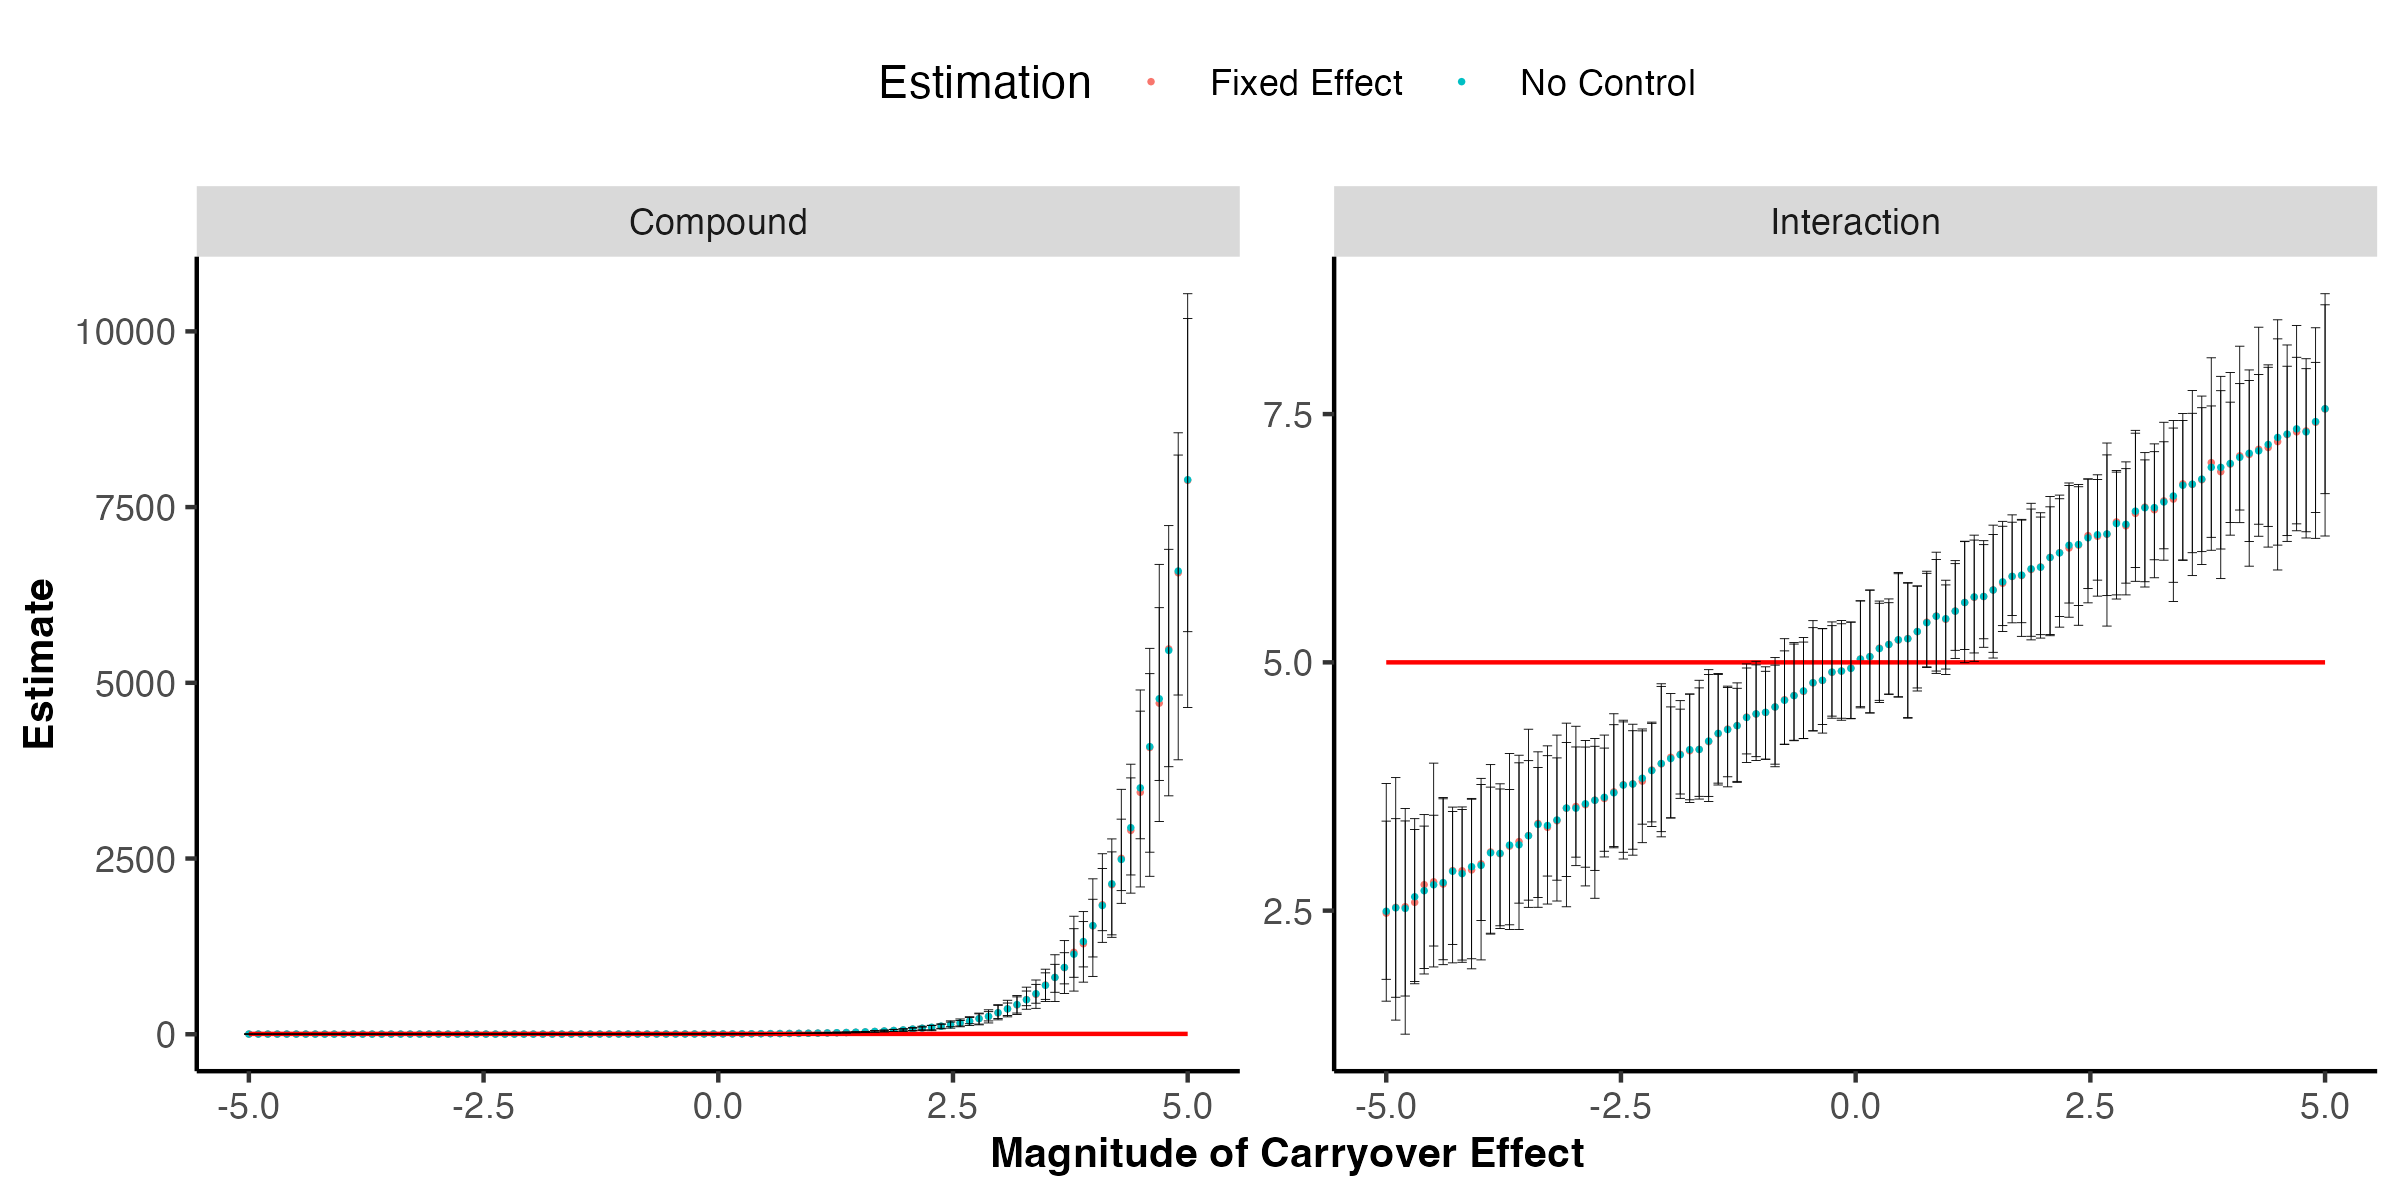
\includegraphics[width=0.95\linewidth]{Figures/CarryoverEffect.png}
    \caption{Simulated estimates of different structures of carryover effects of treatment at $t_1$ on the treatment at $t_2$. On the left, we have the compounding effect (Equation \ref{eq: compounding_carryover}), whereas on the right, we have the simple interaction effect (Equation \ref{eq: interaction_carryover}) between $Z_{t_1}$ and $Z_{t_2}$. The true average treatment effect, $\tau_{\text{ATE}}$, is set at 5 (red horizontal line).}
    \label{fig:simulation_control_carryover}
\end{figure}

Figure \ref{fig:simulation_control_carryover} shows the bias of the estimated treatment effect, $\beta_1$, at $t_2$ varying the magnitude of the carryover effect, $\gamma$, as specified in Model 1 and Model 2. These two examples show how misspecification or ignoring the correct functional form of carryover can bias estimates. In Model 1, adding a simple interaction term can often account for such dependence, whereas in Model 2 requires a different approach to properly estimate the true effect of the second treatment.

\cite{23_AnalysisOfCrossoverTrial} provides an analysis of estimating \cwsd{} (referred to as 2×2 crossover trials) in the case of no carryover effects, as well as additive and interactive carryover effects, using OLS and REML estimators. However, as noted, the functional form of the carryover effect can be difficult to discern, and misspecification can lead to biased estimates.